\documentclass[11pt,twocolumn]{article}
\usepackage{url}
\usepackage{breakurl}
\usepackage[breaklinks]{hyperref}
\usepackage{graphicx}
\usepackage{float}
\begin{document}

\begin{titlepage} % Suppresses displaying the page number on the title page and the subsequent page counts as page 1
    \newcommand{\HRule}{\rule{\linewidth}{0.5mm}} % Defines a new command for horizontal lines, change thickness here
    
    \center % Centre everything on the page
    
    %------------------------------------------------
    %    Headings
    %------------------------------------------------
    
    \textsc{\LARGE Indiana University - Bloomington}\\[1.5cm] % Main heading such as the name of your university/college
    
    \textsc{\Large Network Science}\\[0.5cm] % Major heading such as course name
        
    %------------------------------------------------
    %    Title
    %------------------------------------------------
    
    \HRule\\[0.4cm]
    
    {\huge\bfseries Understanding and Exploring World Happiness Data through Data Visualization and Analysis}\\[0.4cm] % Title of your document
    
    \HRule\\[1.5cm]
    
    %------------------------------------------------
    %    Author(s)
    %------------------------------------------------
    
    \begin{minipage}{0.4\textwidth}
        \begin{flushleft}
            \large
            \textit{Authors}\\
            \textsc{Daniel Hinders\newline} % Your name
            \textsc{Nhi Tran} % Your name

        \end{flushleft}


    \end{minipage}
    ~
    \begin{minipage}{0.4\textwidth}
        \begin{flushright}
            \large
            \textit{Professor}\\
            \textsc{Yong-Yeol (YY) Ahn} % Supervisor's name
        \end{flushright}
    \end{minipage}
    
    % If you don't want a supervisor, uncomment the two lines below and comment the code above
    %{\large\textit{Author}}\\
    %John \textsc{Smith} % Your name
    
    %------------------------------------------------
    %    Date
    %------------------------------------------------
    
    \vfill\vfill\vfill % Position the date 3/4 down the remaining page
    
    {\large\today} % Date, change the \today to a set date if you want to be precise
    
    %------------------------------------------------
    %    Logo
    %------------------------------------------------
    
    %\vfill\vfill
    %\includegraphics[width=0.2\textwidth]{placeholder.jpg}\\[1cm] % Include a department/university logo - this will require the graphicx package
     
    %----------------------------------------------------------------------------------------
    
    \vfill % Push the date up 1/4 of the remaining page
    
\end{titlepage}

\title{Understanding and Exploring World Happiness Data through Data Visualization and Analysis}
\author{Nhi Tran}
\maketitle
\begin{abstract}
Gallup World Poll collected yearly data from 2015 to 2017 to identify the World Happiness ranking of around 155 countries in the world through the six main factors: GPD, Social Support, Life Expectancy, Freedom, Absence of Corruption, Generosity \cite{kaggle-dataset}. The collected data by its raw form is hard to understand with a lot of numbers and ranking for each country's World Happiness factors; therefore, applying visualization would be beneficial and important to fully observe, analyze and understand the provided data in depth.
\end{abstract}

\section{Introduction}
The happiness cores and rankings were created based on data from the Gallup World Poll, which collected people's answers to life evaluation questions. The questions based on the six main factors that contribute to calculating the happiness scores for each country and create a possible method to measure the intangible aspect of life – happiness. The world happiness measurements provide a more positive angle to analyze main life issues and the result is important to help leader evaluate their countries and identify which areas that need improvements to increase people quality of life. 

\subsection{Background}
Gallup is a firm that provides analytics and researches globally to help leaders and organizations make accurate decisions \cite{gallup} . One of their feature projects is creating a World Poll that collects statistics and quantifies the world's happiness level. The results of their yearly World Poll are being utilized and published by multiple organizations such as the World Happiness Report by Sustainable Development Solutions Networks, Bloomberg, The Economist, CNN, etc... \cite{gallup}.

Sustainable Development Solutions Networks published the first World Happiness Report in 2012 with data of roughly 155 countries, and since then, their reports were widely used by experts in all different fields of study to understand human's happiness. 


\subsection{Motivation and Objectives}

The first objective of this analysis is to understand all the different factors that would affect our quality of life. Out of all of the factors, which ones are more important or have a higher proportion than the other? The hypothesis is that GDP per Capita is the most important factor in human happiness. The higher the economy, the better the standard of living, quality of life, and education levels. 

There have been debates between the relationship of GPD per capita and life satisfaction. Some reported no significant relationship between happiness and income; some reported that the relationship exists up to a certain point. According to Eugenio and Aldo's article, the article found that the relationship between GPD per capita and happiness is significant for countries with GPD per capita under \$20,000, while countries with GPD per capita above \$20,000 have much less obvious link \cite{vox}.

Another important objective for this work is to identify countries and/or areas with high improvement and changes in happiness score year over year from 2015 to 2017. This will provide some good benchmark system and insights to observe effective changes, such as changes in government policies, social and healthcare, economic improvement, etc.... 

The last objective is to perform analysis and visualization for any interesting outliers and insights that would be beneficial for happiness improvement. Are there other factors? Would the location of each country affect their happiness level? There have been debates and contradictory on whether weather affects happiness level; A Huffpost article called 'The Surprising Ways The Weather Affects Your Health and Well-Being' stated that Seasonal affect Disorder is a real thing, happiness level can be impacted and people are more likely to be depressed during the colder seasons, however, the article also showed that there are researches indicate that it might be exaggerated \cite{huffpost}. Will the happiness data analysis show a relationship between weather and happiness level?  

Happiness helps people feel better about life and increase creativity and healthy level both physically and emotionally. People with higher happiness level tends to be more successful, live longer and have better social group connections \cite{happiness}. 

All of the findings and analysis from those objectives are essential to increase the world's happiness and help leaderships from all countries making important decisions. Depends on the findings, it might improve the method of ranking and quantifying happiness's levels.


\subsection{Existing Work}
Three interesting existing works use the world's happiness data: The World Happiness Report, Iman Ghosh's post from Visualcapitalist, and Alexander Bastidas Fry's work from his website.

\paragraph{The World Happiness Report \cite{world-happiness-report-2018}} The World Happiness Report in 2018 contains data from 2015-2017 and highlight of the migration issue due to low happiness level. One of the interesting visualizations is the 'Population-Weighted Distributions of Happiness' on page 18 of the report \cite{world-happiness-report-2018}. The visualization used the answers from people valuing their lives from 0 to 10 scale and performed bar charts break down by region to identify the distribution. The strength of this graph is the ability to show the distribution of the data quite clearly. The overall world data, Commonwealth of Independent States, East Asia, Southeast Asia, Middle East, and North Africa have normal distributions, while Northern America \& ANZ, Western Europe, Latin American \& Caribbean, Central, and Eastern Europe have right-skewed distribution and South Asia and Sub-Saharan Africa have left-skewed distribution. That means Northern America and ANZ, Western Europe, Latin American \& Caribbean, Central, and Eastern Europe have a better level of happiness comparing to the world. What this graph is missing is the comparison between the regional distributions, which boxplot does well.

Another interesting visualization from the report is the 'Ranking of Happiness 2015-2017' on page 23, which shows the list of all countries' happiness ranking by ascending order with the breakdown bar charts to show all factors as well as the confidence level \cite{world-happiness-report-2018}. This visualization gives a good overview of all countries along with the composition of the scores. We can briefly notice that GDP, Social Support, and Dystopia Residuals are a large portion of the total score. Dystopia is a benchmark score (this report marked 1.92 as the score, Kaggle source states 1.85) of the most unhappy place on earth, and residual is the other unexplained factors that affect happiness. The idea of Dystopia is to ensure that no country would have a score of 0 or performs worst than Dystopia \cite{kaggle-dataset}. 

Though having impressive visualizations, the work does not concentrate on evidence that supports the objectives of this report. The visualizations narrow the possibility of GDP being a large factor of happiness; however, they do not present the comparison between GDP per capita's contribution to happiness to other factors.
   
\paragraph{Iman Ghosh's Work \cite{visual-capitalist}} The focus of Iman Ghosh's work is visualizing the most and least happy countries around the world in 2019. The main visualization of the world map in her article is very impressive and detailed. The graph shows the score of happiness around the world in high-level effectively and highlights the most and least happiness countries. It is useful to observe and quickly identify if there is an area on the map that performs specifically better or poorer. She then created more visualizations to deep-dive into each region, which are North America, South America, Europe, the Middle East and Central Asia, East Asia, Oceania, and Africa. From the graphic, Oceania is the happiest region; North America performs well on average with Canada being the happiest country and Haiti being the least happy. For each region, the visualizations also include highlighted information or explanation of the countries' score. Africa is the least happy region with Mauritius being the happiest country ranking 57 and Sudan being the least happy. Iman Ghosh also includes a label on the most and least improved country for each region. Iman Ghosh's work helped us analyze the data based on region, as well as identify most improved countries in 2019 such as Nicaragua, Ecuador, Bulgaria, Uzbekistan, Philippines, and Benin.


Iman Ghosh's work was informative and well-graphed, it looks at data in the top and least country level and well as regional level. However, the data are based on a different year as well as do not concentrate on the degree of improvement each country did. We still need to look into the changes year of year to solve one of our objectives. 

Iman Ghosh's world map did help to solve the weather hypothesis. The closer it is to the equator, the hotter the temperature is; however, when looking at the overall map of the happiness score, there is no apparent evidence that the countries around the equator are happier than the countries further away from the equator. It looks like the colder countries (Canada, Australia, Finland, etc...) are happier than the hotter countries. 

\paragraph{Alexander Bastidas Fry's Work \cite{alexander-bastidas-fry}} Alexander's work is the most interactive out of the three existing works on world happiness data. His work has an interactive world map along with scatterplot for each factor. The world map allows a high-level view of the data in 2017 while the scatterplots show the relationship between each factor using a linear regression fit model. Another unique visualization from Alexander's work is the radar plot to allow the prediction data to actual data comparison by the six factors. However, his work lacks the label of Happiness level as well as country's names in the map; it is hard to identify which country ranks the highest based on the visualization and the location of each country by just mainly looking at the map. 

From the scatterplot, the linear regression fit between GDP per Capita and Social Support is the most similar to each other. It indicates that GDP per Capita and Social Support have a very similar trend or relationship to the final happiness score.

This report will differ because one of its objectives is to provide the actual correlation coefficient of the factors as well as the proportion comparison between factors to the total happiness scores.

\section{Process and Approaches}

\begin{figure}[hbt!]
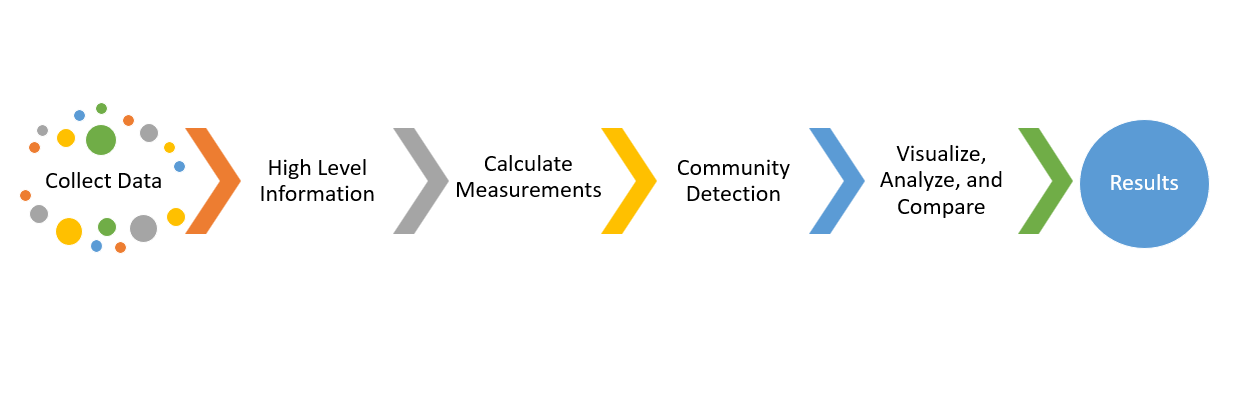
\includegraphics[scale=0.4]{process_flow.PNG} 
\caption{Process cycle}
\end{figure}

\textbf{Figure 1} identifies the steps that are necessary to complete the objectives of this report. Data are collected from Kaggle using Kaggle API. Once the data are collected and well understood, the next step would be to brainstorm all suitable visualization methods to achieve and complete the objectives. It is in the form of a cycle to indicate the possibility of future work to collect more data with more experiments.

\subsection{Data Collecting}

\paragraph{Dataset}
The datasets are 2015-2017 World Happiness Score from Kaggle public dataset. The count of countries collected from 2015-2017 is 158, 157, 155 respectively. The common attributes for all three years datasets are \cite{kaggle-dataset}:
\begin{itemize}
\item \textbf{Country Name} – Name of the country
\item \textbf{Region} – The region where the country belongs to - not available in 2017 data
\item \textbf{Happiness Score} – A metric measured by asking questions: How would you rate your happiness on a scale of 0 to 10 where 10 is the happiest" - It is also the sum of all the factors below.
\item \textbf{Economy (GDP per Capita)} – the extent to which GDP contributes to the calculation of the Happiness Score   
\item \textbf{Family} – the extent to which Family contributed to the calculation of Happiness Score
\item \textbf{Health (Life Expectancy)} – the extent to which Life Expectancy contributed to the calculation of the Happiness Score
\item \textbf{Freedom} – the extent to which Freedom contributed to the calculation of the Happiness Score
\item \textbf{Trust (Government Corruption)} – the extent to which Perception of Corruption contributed to the calculation of the Happiness Score
\item \textbf{Generosity} – the extent to which Generosity contributed to the calculation of the Happiness Score
\item \textbf{Dystopia Residual} – the extent to which Dystopia Residual contributed to the calculation of the Happiness Score
\end{itemize}

\subsection{Data Cleaning}

\paragraph{Tools} Python packages: Jupyter Notebook, Pandas, Matplotlib, Seaborn, Pycountry, Plotly

\paragraph{Tidying} There are no \textit{NaN} or \textit{null} data that needs to be dropped from the dataset. There were some countries with '0.00' value in one of six factors but they do not look like bad data.

The main tidying works are standardizing columns names for all three datasets, performing a join from 2016 data to get the region information for 2017 dataset, and removing unnecessary columns like whisker columns and confidence interval columns.

\subsection{Visualization Methods Brainstorming}

\begin{figure}[hbt!]
\includegraphics[scale=0.3]{brainstorm_visualization.PNG} 
\caption{Visualization Methods Strategy per Objective}
\end{figure}

\textbf{Figure 2} below outlines the visualization methods strategy for each objective. Some of the visualization methods are already created by other existing works, which we can reuse to eliminate repetitive works.

For the first objective, since we want to determine the importance of a certain factor, two things would be interesting to see: proportions and correlation coefficient. 

With proportions, the World Happiness Report's indicates that Social Support, GDP per Capita, and Dystopia Residual are the three main factors of the world's happiness score. However, it would still be essential to see what the actual value of the proportion are and how much does the overall happiness are contributed by GDP per Capita versus the rest of the factors. And since the overall happiness score is the sum of all of the factors and we don't have too many categories, a pie chart would be a good candidate for this problem. 

\subsubsection{Pie Chart} 
\paragraph{Advantage} Pie Chart is great to show proportions between categories, it is easy and simple enough to get the message across \cite{piechart}. 

\paragraph{Disadvantage} Pie Chart should not be used if all of the categories data does not add up to 100\%, it also does not show any other information beside proportion \cite{piechart}.

Alexander's work was able to show us the linear regression fit by using scatterplot between each factor to the happiness score; however, the visualization was lacking the ability to compare the linear regression fit between factors. To further expand Alexander's work, having a capability to show and compare the correlation coefficient between all factors to each other and the final happiness score are beneficial to support the objective. The correlation coefficient is a linear relationship indicator that identifies whether a variable has a positive or negative relationship to the other variable independently. To show multiple correlation values between multiples factors and have the ability to compare them, a visualization method that could show some sort of matrix is what we are looking for. Heatmap is a good candidate to show matrix values with a gradient color scale to show the continuous value of the correlation coefficient.

\subsubsection{Heatmap} 
\paragraph{Advantage} Heatmap utilizes a color scale to show the trends and relationship of data easily.
\paragraph{Disadvantage} Heatmap requires a good understanding of utilizing correct color maps and sometimes it could be too crowded and overflow with information if being used on an incorrect volume of data.

For the second objective, the key is to rank, compare and identify the area of changes in happiness score year over year. To easily find any trend in an area, and we have geographical data, a map is a great candidate and the value would be the changes in happiness score from 2015-2017, therefore, we would have to use gradient color scheme, such as 'Viridis'. Bar charts will also be another candidate to rank and compare the happiness changes year over year as well as showing changes by categories.

\subsubsection{Bar Chart} 
\paragraph{Advantage} Bar Chart is useful to be able to graph and compare a large amount of category data \cite{bar-chart}. In this case, we would like the compare the total amount of each factor and compare to each other to be able to identify the largest category out of the six factors.

\paragraph{Disadvantage} The disadvantage of Bar Chart is the lack of other information such as assumptions, relationships, patterns, etc. \cite{bar-chart}. Therefore, the Bar Chart method will be a good starting point to support other graphs, such as Heatmap or Scatterplot.

\subsubsection{Map} 
\paragraph{Advantage} Map is great for geographical data to display the view of information based on the country or geographic location.
\paragraph{Disadvantage} Sometimes, map graph can be hard to compare or rank the data. Map method can also be misleading sometimes based on the type of data. For example, people tend to display the whole area even though the population is not spread out throughout the whole area \cite{map}. 

The last objective mostly focuses on the ability to identify and visualized outliers and boxplot is a good candidate for outliers. We will also be able to compare the distribution of all factors to see if there are any more new insights. We will have to use and pick colors that are different enough to distinguish the category. A histogram might also be useful to observe the distribution of each factor individually. 

\subsubsection{Boxplot} 
\paragraph{Advantage} It is easy to compare multiple distributions using boxplot and they are useful to show outliers. 
\paragraph{Disadvantage} They do not show as many details of the distribution as a histogram.

\subsubsection{Histogram} 
\paragraph{Advantage} Histogram is useful to show frequency and distribution in a dataset and ensure that data are distributed into equal-sized bins. 
\paragraph{Disadvantage} Histogram requires work to identify the correct amount of bins to show the distribution, sometimes it can be misleading if choosing the wrong bin sizes. They are also hard to compare the distributions between categories.

\subsection{Visualization Experiments and Analysis }
Most of the process of choosing visualization methods and analysis are completed in the attached Python Jupyter Notebook.

The high-level thoughts of the experiments are:

\begin{itemize}
\item Depends on the type of data, most of the categorical graphs such as Pie Chart, box plot utilized qualitative color map while most of the graphs, such as map, heatmap, that show a scale of value works better with gradient color scale. 
\item Boxplot successfully showed the comparison between distributions and gave a lot of information on countries that are outliers.
\item Pie Chart was useful to show the proportion of each factor. The factor, besides Dystopia Residual, that has the largest contribution to the overall Happiness Score are Social Support. 
\item Correlation Coefficients were calculated and displayed using heatmap. Even though half of the matrix is repeated, it was still useful to show some insights on the relationship between variables.
\item Interactive Map was quite tricky, a decision was made to show the country name by hovering instead of displaying labels because it is quite small. However, since it is an interactive map, if zoomed in, we can still map the lists of most improved countries for benchmark and deeper research purpose.
\item One of the bar charts was a failed experiment since it was not able to compare each category. From the failed experiment, a different approach was to calculate the changes and display them on a bar chart instead.
\item Another failed experiment was the world map that displayed the changes from 2015-2017. It worked well in a sense that gives us an idea of the area that has the most improved happiness countries; however, it does not work well sho

\item An interesting activity was to split the data into 4 small datasets based on the quartiles value of happiness score and see if the correlation coefficient changes based on different groups of happiness score. 
\end{itemize}
\section{Results and Insights}
\subsection{Objective 1 - How important is GDP per Capita toward Happiness Score?}
From the pie chart and heatmap visualizations, it is confirmed that GDP has a large percentage(around 18.4\%) in the overall happiness score. However, GDP is not the most important factor. Social Support and Life Expectancy also are very important in the total Happiness Score.
\subsection{Objective 2 - Which countries/areas are the most improved countries between 2015 and 2017?}
Some countries were dropped during this visualization process because they are either not in 2015 dataset or 2017 dataset. The improved countries from 2015 to 2017 in descending order are Latvia, Romania, Togo, Senegal with 0.752, 0.701, 0.656, 0.631 increase in Happiness Score respectively. 

From 2015 to 2017, the most improved factor in Latvia is Dystopia Residual (around 0.37 increase), followed by Social Support (around 0.31 increase) and then GDP per Capita (0.15 increase). The central area of the map contains the highest counts of improved countries.

\subsection{Objective 3 - Other Insights and Outliers}
Some of the most important outliers are:

- Poor performance in Social Support: Benin, Syria, Central African Republic

- Great performance in Generosity: Myanmar, Indonesia

- Great performance in Government Trust: Singapore, Qatar, Denmark, Sweden, Switzerland, United Arab Emirates, Australia, Ireland

- Great performance in Dystopia Residual: Somalia

- Poor performance in Dystopia Residual: Tanzania, Hong Kong, Sri Lanka, Botswana 

Some other insights are involved in the correlation coefficient data. When looking at the whole dataset, GDP per capita, social support, and life expectancy are the three factors that have the highest relationship to the overall happiness score. GDP per Capita, social support, and life expectancy also have a high correlation with each other, surprisingly. There is also a correlation between government trust and freedom.

When splitting the Happiness Data into 4 datasets based on the Happiness Score quartiles, we noticed that GDP per Capita and Social Support were the main variables with high correlation for 1st quartile dataset. However, when we look at the second quartile dataset, the relationship is no longer dominated by GDP per Capita and Social Support. Life Expectancy and Freedom correlation increased and become about the same as GDP per Capita and Social Support. In the third quartile, however, Life Expectancy's correlation is no longer comparable to GDP per Capita, Social Support, and Freedom. Lastly, in the fourth quartile, GDP per capita is no longer high on the correlation coefficient. Social support, life expectancy, freedom, generosity, and government trust are the five factors with a high correlation. 

The other generic insights are:

- Countries are more likely to have low Generosity contribution and Government Trust Contribution

- Happiness Score has a normal distribution

- There are a lot of countries that have high social support.

\section{Discussion}
From the results section, besides Dystopia Residual, social support is the factor with the second-highest improvement in Latvia from 2015 - 2017. It urges a question 'What did Latvia do between 2015 and 2017 related to Social Support that caused the contribution to Happiness Score increase?  

According to the BTI project website, Latvia made some great international decision and joined multiple major western international organization \cite{bti-latvia}. Latvia also kept a balanced budget, its government focused more on reforming the economy, tax system, healthcare financing, and school system \cite{bti-latvia}. Those could be some of the indicators of why there was an increase in social support contributes to the country's happiness score.

Another piece of insights is Myanmar being the highest performer in Generosity. Why is it? According to a Devex article, Myanmar has been in the top of the World Giving Index for the previous couple years before 2014 \cite{myanmar}. The article suggests that it is since Myanmar has a high proportion of Theravada Buddhists.

There are many opportunities for future work based on the results of this report. A lot of research is still needed on countries that were outliers or countries that perform well year over year. There are still also more analysis needed on the reasons why there is a difference in the correlation coefficient between quartiles. Regions were also another piece of data that were never being considered in this report that could give great insights. Another question that was not answered is whether GDP has a lesser effect in countries with more than \$20,000 income. The dataset is too high-level to answer that question. 

\section{Conclusion}
The visualization methods are very useful in data analysis and provide a lot of insights from raw data. Most of the results are beneficial and could be treated as starting points for more in-depth study and statistical modeling to determine how we could increase the happiness level. This report also encourages the search for the data that results in this dataset to be able to perform analysis on a more granular data. 

One of the potential future work would be doing more visualizations such as scatterplot to determine why the correlation coefficient changed dramatically between different happiness score quantiles datasets. 

\section{Acknowledgment}
Special thanks to Professor Yong-Yeol Ahn and his TA Nathan Ratkiewicz for teaching the Data Visualization class and introducing multiple topics and techniques in visualization
\section{References}
\bibliography{references} 
\bibliographystyle{ieeetr}
\end{document}
